\section{Introduction}\label{sec:intro}
\epigraph{If you would understand anything, observe its beginning and its development.}{Aristotle}

Questions regarding the history of data visualization are (or at least should be) of great importance to historians of science, to current developers of graphical methods for statistical analysis and the related info-vis community, as well those just interested in the history of ideas. In the history of science, diagrams, graphs, maps and other visualizations have often played important roles in discoveries that arguably might not have been achieved otherwise.%
\footnote{
	Some salient examples are:
	Francis Galton's 1861 discovery of anti-cyclonic movement of wind around low-pressure areas from contour maps; Edward Maunder's ``butterfly diagram'' of the variation of sunspots over time leading to the	discovery of the ``Maunder minimum,'' from 1645--1715; and Henry Moselely's 1913 discovery of the concept of atomic number, based largely on graphical analysis (a plot of serial numbers of the elements vs. square root of frequencies from their X-ray spectra).
}
At the same time, in the fields of statistical graphics and information visualization, developers often create ``new'' methods without any appreciation that they have deep roots in the past.%
\footnote{
  For example, mosaic displays for frequency tables were thought to have been invented by \citet{HartiganKleiner:81} and extended to show the pattern of residuals in loglinear models by \citet{Friendly:94a}. But it turns out that the essential idea behind this area-based display is goes back to Georg von Mayr in 1877 \citep{Friendly:2002:mosahist}.
}

These two perspectives provided the motivation for the development of the Milestones Project. 
\begin{comment}
Rephrase the second sentence: Previous historical accounts of events, ideas and techniques that relate \emph{inter alia} to modern data visualizations were fragmented - scattered across a wide number of fields, publications, and languages (insert footnote here).  The present project's goal was to bring these resources together into a publicly and freely available database.
\end{comment}
This stemmed from the fact that historical accounts of events, ideas and techniques that relate \emph{inter alia} to modern data visualization were fragmented and scattered across a wide number of fields.%
\footnote{
Among these are general histories in the fields of probability \citep{Hald:1990}, statistics \citep{Pearson:1978,Porter:1986,Stigler:1986}, astronomy \citep{Riddell:1980}, cartography \citep{WallisRobinson:87}. More specialized accounts focus on the early history of graphic recording \citep{HoffGeddes:1959,HoffGeddes:1962}, statistical graphs \citep{Funkhouser:1936,Funkhouser:1937,Royston:1970,Tilling:1975}, fitting equations to empirical data \citep{Farebrother:1999}, cartography \citep{Friis:1974,Kruskal:1977}, thematic mapping \citep{FriendlyPalsky:2007,Palsky:1996,Robinson:1982}, and so forth.
}

When this work began in the mid-1990s, there were no accounts or resources that spanned the entire development of visual thinking and the visual representation of data across different disciplines and perspectives. The Milestones Project began simply as an attempt to collate these diverse contributions into a single, comprehensive listing, organized chronologically, that contained representative images, references to original sources, and links to further discussion -- a source for ``One-Stop Shopping'' on the history of data visualization.

In \secref{sec:project}, we describe the evolution and structure of the Milestones Project. \secref{sec:vistime} presents some historical and modern approaches to one self-referential question: how can data visualization be applied to its own history? \secref{sec:historiography} introduces another self-referential topic we call \emph{statistical historiography}, which entails the use of statistical and graphical methods for the analysis and understanding of historical innovations, developments, and trends. But first we give some brief vignettes of historical topics and questions for which the Milestones Project has proved invaluable in our own research.

\begin{comment}
These have all been dealt with
\begin{itemize*}
 \item The first statistical graph?
 \item Who invented the scatterplot?
 \item The origin of mosaic displays
 \item The Golden Age of statistical graphics
\end{itemize*}
\end{comment}

\subsection{The first statistical graph}
In the history of statistical graphics \citep{Friendly:06:hbook}, as in other artful sciences, there are a number of inventions and developments that can be considered ``firsts'' in these fields. The catalog of the Milestones Project \citep{FriendlyDenis:01} lists 70 events that can be considered to be the initial use or statement of an idea, method or technique that is now commonplace, but there is probably no question more fundamental than that of the first visual representation of statistical data.

In \citet{Friendly-etal:2010:langren} we argue that the 1-dimensional line graph shown in \figref{fig:langren-google-overlay} by Michael Florent van Langen \citep{Langren:1644} should be accorded this honour. The graph shows 12 estimates of the distance in longitude between Toledo and Rome, overlaid on a modern map. van Langren used this to demonstrate that these estimates were all subject to large errors and to
propose to King Phillip of Spain that only he had a sufficiently precise method for the determination of longitude for navigation at sea.

\begin{figure}[htb]
 \centering
 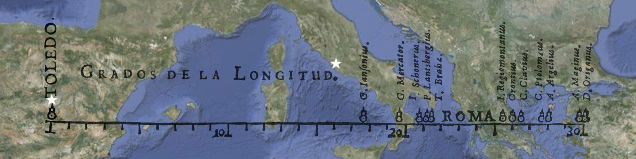
\includegraphics[width=\textwidth]{fig/langren-google-overlay2}
 \caption{van Langren's 1644 graph, re-scaled and overlaid on a modern map of Europe. Toledo is located at lat/long %39$^o$51$^'$36$^\"$N, 4$^o$01$^'$48$^\"$W
(\degree{+39.86}N, \degree{-4.03}W), Rome is located at (\degree{+41.89}N, \degree{+12.5}W), both shown by markers (stars) on the map.  This image makes clear what van Langren wished to communicate: the wide variability of the estimates, but also shows how far the estimates were biased.}%
\label{fig:langren-google-overlay}
\end{figure}

The telling of van Langren's story not only turned out to involve astronomy, archival research, the history of patronage in the \Cent{17}, and even an unsolved problem of cryptography, but also serves as an example of statistical historiography.  The Milestones Project provided the infrastructure for this research -- through the use of a time-based, cross-referenced catalog of images, references and links to related work, van Langren's tale was able to be studied and reported upon.

\subsection{Who invented the scatterplot?}
%\TODO{MF: Revert or merge some of this text with the version as of 29 Aug... }
Although there are earlier precursors, the main graphical methods used today---
pie charts, line graphs and bar charts--- are generally attributed to
William Playfair in works around the beginning of the \Cent{19}
\citep{Playfair:1786,Playfair:1801}. All of these are essentially univariate
displays of some aspect of a single variable. 

A logical next step would be to invent a method to reveal the relationship between two variables--- what we now know as the scatterplot.  By \citeyear{Galton:1886}, Francis Galton had utilized this truly bivariate display, which led to the
discovery of correlation and regression, and ultimately to much of present multivariate
statistics. 
However, he was not the first to use this graphical technique, and it is surprising that no one is widely credited with its invention.

In \citet{FriendlyDenis:05:scat}, we delved into this mystery.  This involved tracing the early origins of ideas related to the scatterplot, which led to two compelling narratives: how, in Playfair's time, it was nearly impossible to think about and visualize bivariate relationships; and, later, how the scatterplot was essential for Galton's visual insights that would lead to the rise of modern statistics and graphics. It was the resources available in the Milestones Project that allowed us to focus upon the events in this period and attribute the essential ideas of the scatterplot to J. F. W. Herschel in two 1832 papers.

\subsection{The Golden Age of statistical graphics}

In our initial web presentation of the Milestones Project, it proved convenient
to sub-divide the history of data visualization into epochs, each of which turned
out to be describable by coherent themes.  As we illustrate later, one
period turned out to be particularly noteworthy, both for the sheer number of
contributions, and for the beauty and elegance of their execution. We call this period, from roughly 1850 to 1900 ($\pm 10$), the Golden Age of statistical graphics \citep{Friendly:2008:golden}.

\figref{fig:mileyears4} shows the time distribution of the 260 significant events that had been included in the Milestones Project database by 2007, demarcated by the labels we used for epochs. In \citet{Friendly:2008:golden}, we traced the origin of this period in terms of the infrastructure required to produce such an explosive growth of contributions to data visualization, and found three primary sources: the systematic data collection by state agencies, the rise in popularity of statistical and visual thinking, and the enabling developments of technological innovations.
%% one figure
\begin{figure}[!htb]
  \centering
  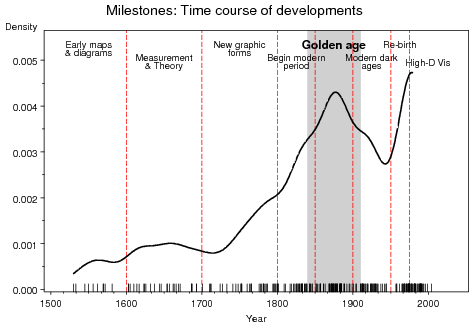
\includegraphics[width=.9\textwidth,clip]{fig/mileyears4}
  \caption{The time distribution of events considered milestones in the history of data visualization, shown by a rug plot and density estimate. The density estimate is based on $n=260$ significant events in the history of data of data visualization from 1500--present. The developments in the highlighted period, from roughly 1840--1910 comprise the Golden Age of statistical graphics.}
  \label{fig:mileyears4}
\end{figure}